\capitulo{5}{Aspectos relevantes del desarrollo del proyecto}

\section{Arquitectura general del sistema}

Uno de los aspectos más importantes del proyecto ha sido el diseño de una arquitectura modular que permitiera separar claramente las distintas responsabilidades del sistema.

La solución desarrollada se compone de varios módulos independientes que trabajan de forma coordinada para procesar los eventos generados en el entorno simulado. Esta división facilita el mantenimiento del código y permite futuras ampliaciones sin necesidad de modificar el funcionamiento del resto de componentes.

El flujo de funcionamiento del sistema comienza con la generación de eventos por parte de los distintos dispositivos simulados. Estos eventos son procesados por el módulo de ingesta, que se encarga de leer y normalizar la información recibida.

Posteriormente, los eventos son almacenados en una base de datos SQLite y analizados por el motor de correlación y detección de anomalías. Finalmente, la información se pone a disposición de los usuarios mediante una API REST desarrollada con FastAPI y un dashboard web implementado con Streamlit.

La arquitectura general del sistema se muestra en la Figura \ref{fig:img/siem_flujo}, presentada en el Capítulo 3.

Se optó por la arquitectura modular basada en componentes independientes. Esta decisión permitió desarrollar y validar cada módulo de forma aislada antes de integrarlo con el resto del sistema. El resultado final es una solución compuesta por un módulo de ingesta, una base de datos SQLite, un motor de correlación, un módulo de detección de anomalías, una API REST y un dashboard de monitorización.

\section{Diseño del entorno simulado}

Con el objetivo de disponer de un escenario realista para validar el funcionamiento del sistema SIEM, se diseñó un entorno simulado basado en un polvorín militar destinado al almacenamiento de material sensible.

El entorno incluye diferentes depósitos distribuidos dentro de un recinto protegido por sistemas de seguridad física y ambiental. Cada uno de los depósitos incorpora distintos dispositivos capaces de generar eventos relevantes para el sistema de monitorización.

Entre los elementos simulados se encuentran los sistemas de control de acceso mediante tarjeta identificativa, sensores magnéticos de apertura de puertas, sensores volumétricos de movimiento, cámaras de vigilancia perimetral, sensores de temperatura y humedad, así como sistemas de alimentación eléctrica respaldados mediante grupo electrógeno.

La utilización de un entorno simulado ha permitido representar situaciones potencialmente críticas sin necesidad de acceder a instalaciones reales ni utilizar información sensible. Además, este enfoque facilita la generación controlada de eventos para validar el correcto funcionamiento del sistema desarrollado.

\imagen{img/plano_polvorin}
{Plano general del entorno simulado utilizado para la validación del sistema SIEM.}
{0.90}

El entorno simulado está compuesto por un total de 20 depósitos de almacenamiento identificados mediante los códigos D01 a D20, distribuidos dentro de un recinto protegido por diferentes medidas de seguridad física. El acceso principal dispone de un torno de entrada y un sistema de control de acceso mediante tarjeta identificativa para regular el acceso al interior de la instalación.

La seguridad perimetral se complementa mediante un vallado de protección, cámaras de vigilancia distribuidas por el recinto y torres de vigilancia situadas en puntos estratégicos. Cada uno de los depósitos incorpora sensores magnéticos de apertura de puertas, sensores de movimiento y sensores ambientales encargados de monitorizar la temperatura y la humedad.

Adicionalmente, el entorno dispone de un edificio técnico destinado a la gestión de los sistemas de monitorización, dependencias auxiliares para el personal, un hangar para vehículos y un sistema de respaldo eléctrico mediante grupo electrógeno. Todos estos elementos generan eventos que son procesados por el sistema SIEM para realizar tareas de monitorización, correlación y detección de anomalías.

La combinación de estos elementos permite disponer de un escenario suficientemente realista para evaluar el comportamiento del sistema desarrollado ante diferentes situaciones de seguridad, tanto relacionadas con el control de accesos como con las condiciones ambientales o el funcionamiento de los distintos dispositivos desplegados.

El sistema desarrollado permite monitorizar eventos, generar alertas y proporcionar una visión centralizada del estado de seguridad del entorno monitorizado. Sin embargo, al tratarse de una solución SIEM, sus capacidades se limitan a la recopilación, análisis y visualización de información.

Por tanto, el sistema no puede actuar físicamente sobre la infraestructura protegida, no siendo capaz de bloquear accesos, cerrar puertas, restringir la entrada al polvorín ni ejecutar acciones de respuesta automática sobre los dispositivos desplegados. Estas actuaciones corresponderían a sistemas de control físico o automatización externos.

\section{Diseño del formato de eventos}

Uno de los aspectos más importantes del proyecto ha sido la definición de un formato de eventos común para todos los dispositivos simulados.

El objetivo de esta normalización es garantizar que la información procedente de diferentes fuentes pueda ser procesada de forma homogénea por el sistema SIEM.

Cada evento generado incluye información relacionada con la fecha y hora del suceso, origen del evento, tipo de evento, nivel de criticidad, usuario implicado, punto de acceso, depósito afectado, dispositivo generador, resultado de la operación y una descripción detallada del evento.

La estructura final utilizada permite disponer de información suficiente para realizar búsquedas, correlaciones y análisis posteriores de manera eficiente.

Esta normalización simplifica además el almacenamiento de los eventos dentro de la base de datos y facilita futuras ampliaciones del sistema.

\section{Implementación del módulo de ingesta}

El módulo de ingesta es el encargado de procesar los eventos generados dentro del entorno simulado.

Su función principal consiste en leer los registros almacenados en los archivos de logs, validar que cumplen el formato definido y transformar la información en estructuras internas que puedan ser utilizadas por el resto de componentes del sistema.

Durante el desarrollo fue necesario implementar mecanismos capaces de gestionar eventos incompletos o mal formados, evitando que errores puntuales afectasen al funcionamiento global del sistema.

Una vez procesados, los eventos son enviados a la base de datos para su almacenamiento y posteriormente utilizados por los módulos de correlación y detección de anomalías.

La separación de este componente respecto al resto del sistema facilita la incorporación futura de nuevas fuentes de información sin necesidad de modificar el resto de la arquitectura.

\section{Implementación del motor de correlación}

Una de las funcionalidades principales de un sistema SIEM es la capacidad de correlacionar eventos procedentes de diferentes fuentes con el objetivo de detectar posibles incidentes de seguridad.

Para este proyecto se ha desarrollado un motor de correlación basado en reglas sencillas que analiza los eventos almacenados y genera alertas cuando se cumplen determinadas condiciones previamente definidas.

Entre las reglas implementadas se encuentran la detección de accesos denegados repetidos, accesos realizados fuera del horario permitido, anomalías ambientales y situaciones de actividad elevada en determinados depósitos.

Durante el desarrollo se implementaron además reglas específicas para detectar aperturas de puertas, movimiento en zonas protegidas, temperaturas superiores a los límites configurados, niveles de humedad fuera de rango y fallos en dispositivos o sistemas de alimentación eléctrica. Cada una de estas situaciones genera alertas clasificadas según su nivel de criticidad.

Cuando una regla se activa, el sistema genera una alerta que queda registrada en la base de datos y posteriormente puede ser consultada a través de la API o visualizada en el dashboard.

La utilización de reglas permite adaptar fácilmente el comportamiento del sistema a diferentes escenarios de seguridad mediante la incorporación de nuevas condiciones sin necesidad de modificar el resto de componentes.

\section{Detección de anomalías}

Además de las reglas de correlación, el sistema incorpora un módulo específico de detección de anomalías destinado a identificar comportamientos potencialmente anómalos dentro del entorno monitorizado.

El análisis realizado se basa en la evaluación de diferentes tipos de eventos y condiciones de funcionamiento. Entre las anomalías detectadas se encuentran temperaturas fuera de rango, niveles de humedad anómalos, accesos fuera de horario, múltiples accesos denegados y niveles de actividad inusualmente elevados en determinados depósitos.

Cada anomalía detectada recibe una puntuación de riesgo (\textit{risk score}) que permite clasificarla según su gravedad. Esta puntuación facilita la priorización de incidentes y permite identificar rápidamente aquellas situaciones que requieren una atención inmediata.

Las anomalías detectadas se presentan en el dashboard ordenadas por nivel de criticidad, proporcionando una visión clara del estado general del sistema.

Aunque inicialmente se valoró la utilización de técnicas de aprendizaje automático (Machine Learning), finalmente se optó por una solución basada en reglas. Esta decisión se tomó debido al alcance académico del proyecto y a la necesidad de disponer de un sistema ligero, fácilmente interpretable y sencillo de mantener. El enfoque adoptado permite detectar situaciones potencialmente anómalas sin necesidad de entrenar modelos ni disponer de grandes volúmenes de datos históricos.

\section{Base de datos SQLite}

Para el almacenamiento persistente de la información se ha utilizado una base de datos SQLite. La elección de esta tecnología se debe a su sencillez de uso, reducido consumo de recursos y facilidad de integración con aplicaciones desarrolladas en Python.

La base de datos almacena tanto los eventos generados por los distintos dispositivos simulados como las alertas producidas por el motor de correlación. Esta información puede ser consultada posteriormente mediante la API REST o visualizada desde el dashboard de monitorización.

Durante el diseño se optó por una estructura sencilla compuesta por tablas específicas para eventos y alertas. Esta aproximación permite mantener una organización clara de la información y facilita futuras ampliaciones del sistema.

La utilización de SQLite resulta especialmente adecuada para un sistema SIEM ligero como el desarrollado en este proyecto, ya que evita la necesidad de desplegar servidores de bases de datos adicionales y simplifica considerablemente la instalación y mantenimiento de la solución.

La estructura de la base de datos se compone principalmente de dos tablas: una tabla de eventos, donde se almacenan los registros normalizados procedentes de los distintos dispositivos simulados, y una tabla de alertas, donde se guardan las alertas generadas por el motor de correlación. Las anomalías mostradas en el dashboard se obtienen a partir del análisis de los eventos y alertas registrados por el sistema.

Las Figuras siguientes muestran ejemplos de registros almacenados en las tablas principales de la base de datos utilizadas por el sistema.

\imagen{img/sqlite_alerts}
{Registros almacenados en la tabla de alertas generadas por el sistema.}
{0.90}

\imagen{img/sqlite_events}
{Registros almacenados en la tabla de eventos normalizados.}
{0.90}


\section{Desarrollo de la API REST}

Con el objetivo de facilitar el acceso a la información almacenada por el sistema, se desarrolló una API REST utilizando el framework FastAPI.

La API actúa como elemento de comunicación entre la base de datos y el dashboard de monitorización, permitiendo consultar eventos, alertas, estadísticas y estado de los sensores mediante peticiones HTTP.

Entre los servicios implementados destacan los destinados a la obtención de estadísticas generales, consulta de eventos recientes, visualización de alertas, monitorización de sensores y detección de anomalías.

La utilización de una API independiente proporciona una arquitectura más flexible y facilita la integración futura con otras aplicaciones o sistemas externos.

\begin{figure}[htbp]
	\centering
	
	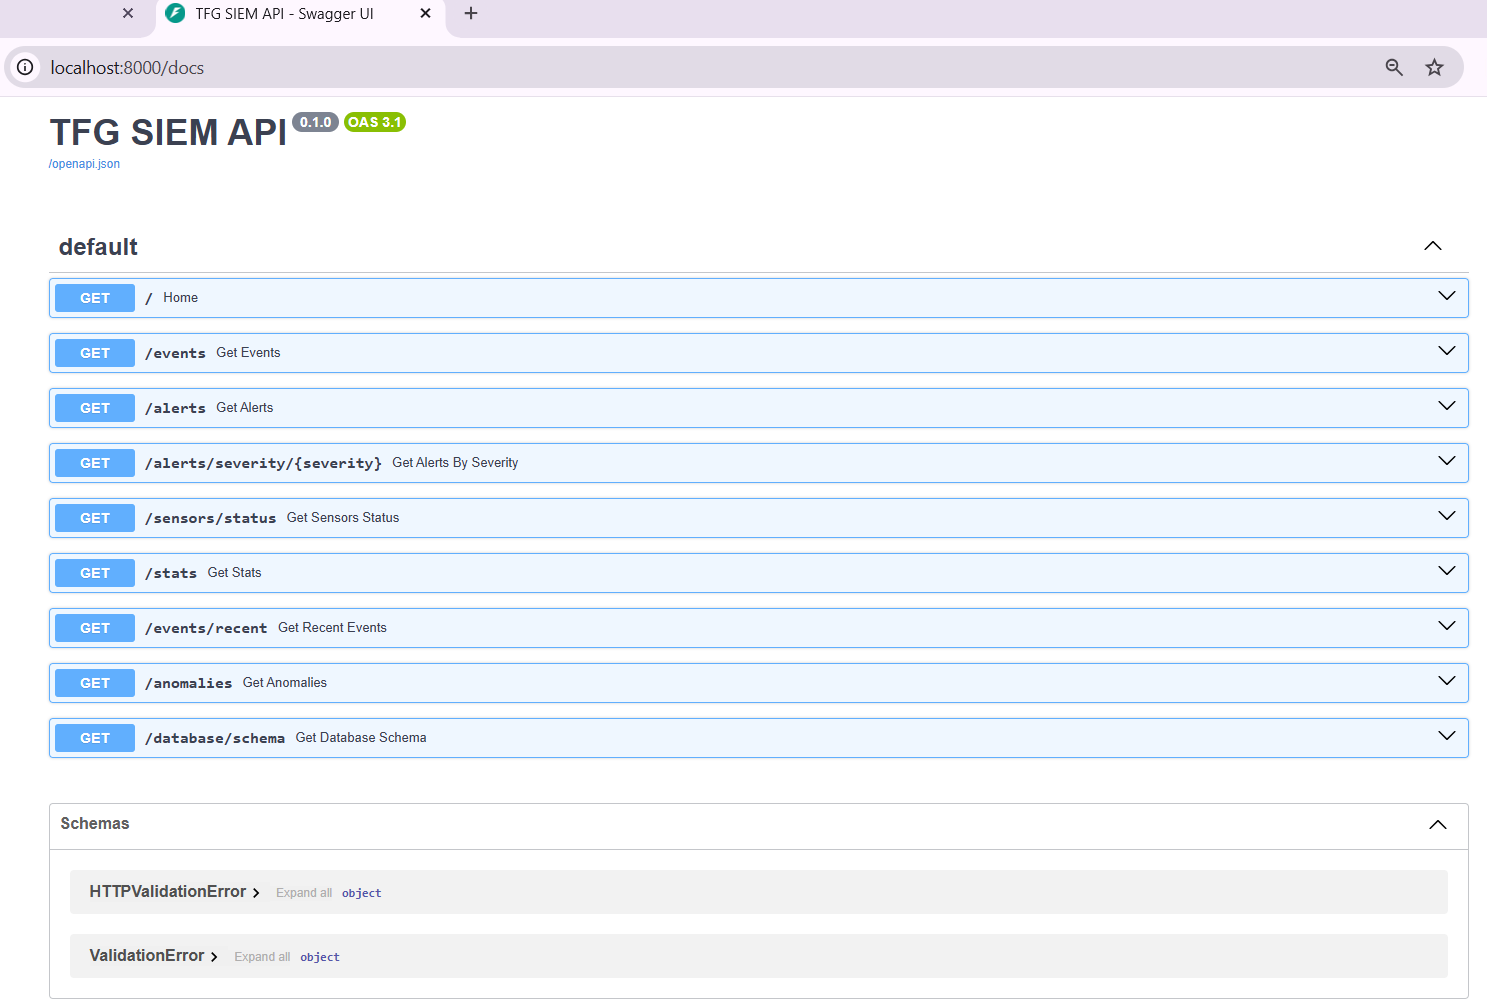
\includegraphics[width=0.85\textwidth]{img/swagger_api.png}
	
	\vspace{0.3cm}
	
	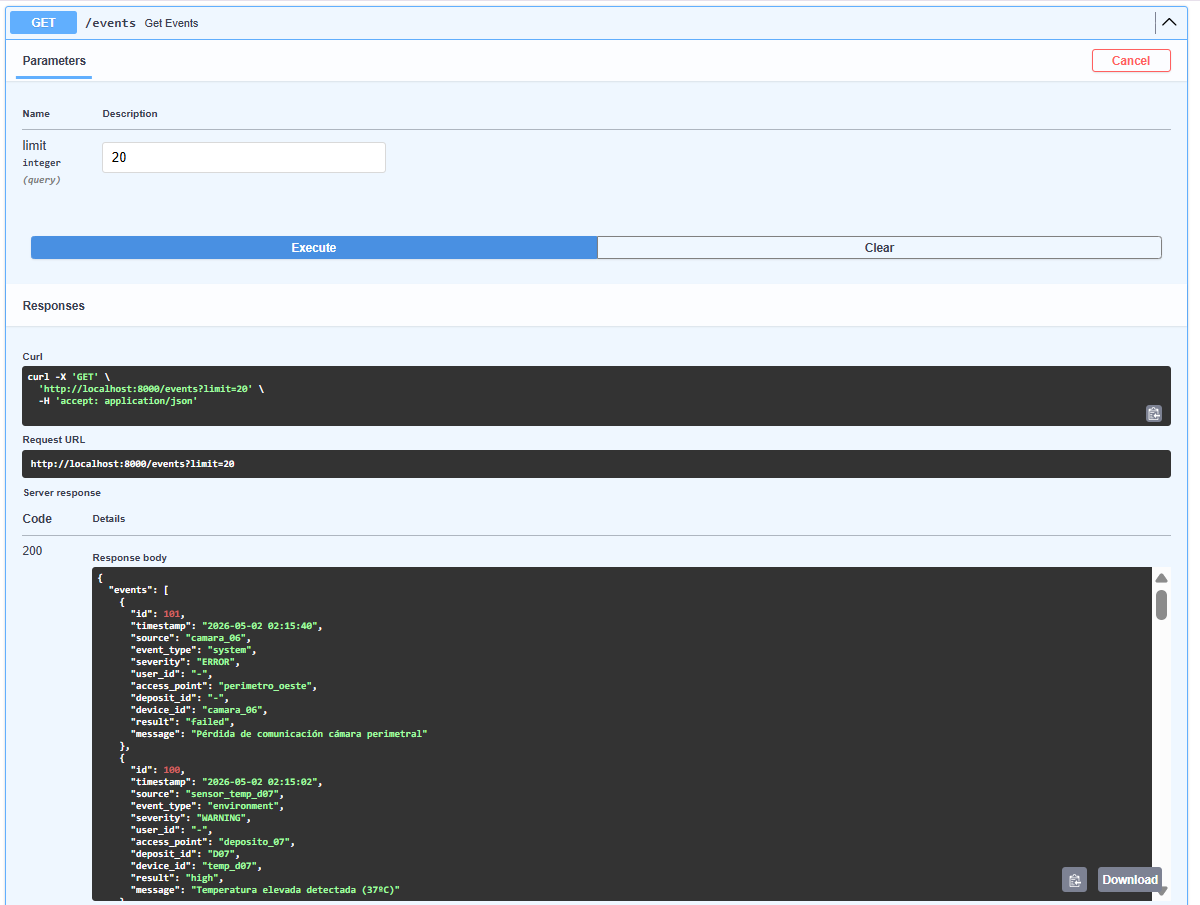
\includegraphics[width=0.85\textwidth]{img/swagger_events.png}
	
	\caption{Documentación Swagger y ejemplo de consulta realizada sobre la API REST.}
	\label{fig:swagger}
\end{figure}

La documentación de la API se genera automáticamente mediante Swagger. Además de mostrar los endpoints disponibles, permite ejecutar consultas y visualizar las respuestas obtenidas directamente desde el navegador.

\section{Desarrollo del dashboard de monitorización}

Para la visualización de la información se desarrolló una interfaz web utilizando Streamlit. El objetivo principal del dashboard es proporcionar una visión clara y centralizada del estado del sistema, permitiendo consultar de forma rápida los eventos registrados, las alertas generadas y el estado de los dispositivos monitorizados.

Durante el desarrollo se diseñó una estructura dividida en varias páginas con el fin de mejorar la organización de la información y facilitar la navegación del usuario. Esta división permite acceder de forma independiente a los diferentes elementos del sistema sin sobrecargar una única pantalla con toda la información disponible.

La página principal muestra información general sobre el funcionamiento del SIEM, incluyendo estadísticas, actividad reciente, alertas generadas y anomalías detectadas.

\imagen{img/dashboard_principal}
{Vista general de la página principal del dashboard de monitorización.}
{0.90}

La página principal muestra el estado general del sistema, estadísticas de eventos y alertas, así como un resumen de las anomalías detectadas.

\imagen{img/dashboard_principal2}
{Resumen de anomalías detectadas y clasificación según nivel de riesgo.}
{0.90}

\imagen{img/dashboard_principal3}
{Actividad reciente registrada por el sistema SIEM.}
{0.90}

Adicionalmente, se desarrollaron páginas específicas destinadas a la consulta de eventos y alertas.

\imagen{img/dashboard_2alertas}
{Consulta de alertas generadas por el motor de correlación.}
{0.90}

\imagen{img/dashboard_2alertas2}
{Distribución de alertas clasificadas según su nivel de criticidad.}
{0.80}

\imagen{img/dashboard_2eventos}
{Listado de eventos registrados por el sistema.}
{0.90}

\imagen{img/dashboard_2eventos2}
{Representación gráfica de la distribución de eventos por tipo.}
{0.80}

También se desarrollaron páginas específicas para la monitorización de sensores y la configuración de parámetros del sistema.

\imagen{img/dashboard_3sensores}
{Monitorización del estado de los sensores desplegados en el entorno simulado.}
{0.90}

La monitorización de sensores permite conocer en tiempo real el estado operativo de los distintos dispositivos integrados en el entorno simulado. El sistema identifica aquellos sensores que se encuentran activos y transmitiendo información con normalidad, así como los dispositivos que permanecen inactivos o que no han enviado eventos durante el intervalo de tiempo configurado.

Con el objetivo de simular situaciones reales de operación y mantenimiento, algunos sensores se mantienen definidos en estado inactivo. Esto permite validar la capacidad del SIEM para detectar dispositivos fuera de servicio, fallos de comunicación o futuras ampliaciones de la infraestructura monitorizada, funcionalidad habitual en entornos reales de supervisión de seguridad.

Además de las funciones de monitorización, el dashboard incorpora una sección de configuración que permite modificar distintos parámetros operativos sin necesidad de realizar cambios en el código fuente. Entre ellos se encuentran los límites ambientales, los horarios permitidos de acceso, los tiempos máximos de inactividad de sensores y los criterios utilizados para la generación de alertas críticas.

Los umbrales de temperatura y humedad configurados en el sistema se han definido con fines de simulación tomando como referencia recomendaciones generales de conservación de materiales sensibles y los principios de protección ambiental recogidos en documentación OTAN relativa al almacenamiento de municiones y explosivos. Estos límites permiten generar eventos de monitorización ambiental y validar el funcionamiento del sistema SIEM ante condiciones potencialmente anómalas.


\imagen{img/dashboard_3configuracion}
{Panel de configuración que permite modificar los umbrales de funcionamiento y los parámetros de monitorización del sistema.}
{0.90}

Entre las funcionalidades incorporadas destacan los filtros por depósito y criticidad, la representación gráfica de eventos y alertas, la clasificación de anomalías por nivel de riesgo y la supervisión del estado de los dispositivos monitorizados.

Como complemento al sistema de monitorización, se implementó un mecanismo de notificaciones SMS simuladas para alertas críticas. Aunque no se realiza el envío real de mensajes, esta funcionalidad permite representar cómo actuaría el sistema ante incidentes de elevada criticidad, facilitando futuras ampliaciones orientadas a la integración con servicios reales de mensajería o notificación.

\imagen{img/dashboard_3sms}
{Configuración de la simulación de notificaciones SMS para alertas críticas.}
{0.90}

Aunque las notificaciones se encuentran simuladas, la arquitectura desarrollada permite sustituir fácilmente este mecanismo por servicios reales de mensajería o plataformas de notificación externas sin necesidad de modificar el resto de componentes del sistema.

Estas características permiten disponer de una visión global del sistema y facilitan la identificación rápida de posibles incidencias de seguridad dentro del entorno monitorizado.

\section{Problemas encontrados y soluciones adoptadas}

Durante el desarrollo del proyecto surgieron diferentes dificultades técnicas que obligaron a replantear algunas decisiones iniciales y a realizar modificaciones sobre la arquitectura del sistema.

Uno de los primeros problemas detectados estuvo relacionado con el formato de los eventos. Inicialmente se utilizó una estructura de logs más sencilla, pero a medida que avanzó el desarrollo se comprobó que la información disponible resultaba insuficiente para realizar correlaciones complejas. Como solución se amplió el formato incorporando campos adicionales como el identificador del usuario, punto de acceso, depósito afectado, dispositivo generador y resultado de la operación.

Otro aspecto que requirió varias modificaciones fue la detección de anomalías. Las primeras versiones se limitaban a identificar condiciones muy concretas, lo que dificultaba la priorización de incidentes. Para solucionar esta limitación se incorporó un sistema de puntuación de riesgo (\textit{risk score}) que permite clasificar las anomalías según su gravedad y mostrarlas ordenadas dentro del dashboard.

También surgieron dificultades relacionadas con la monitorización de sensores. Inicialmente el sistema únicamente mostraba los dispositivos que habían generado eventos recientes. Sin embargo, esta aproximación impedía conocer el inventario completo de sensores existentes. Para resolver este problema se desarrolló un sistema de inventario capaz de representar tanto los dispositivos activos como aquellos que no habían comunicado información recientemente.

Durante el desarrollo del dashboard se realizaron varias reorganizaciones de la interfaz. Las primeras versiones concentraban toda la información en una única pantalla, lo que dificultaba la navegación cuando aumentaba el volumen de datos. Finalmente se optó por dividir la aplicación en varias páginas diferenciadas, separando la información general, los eventos y alertas, y la gestión de sensores y configuración.

Otra dificultad encontrada estuvo relacionada con la calidad del código. Durante las fases finales del desarrollo se utilizó la herramienta Codacy para analizar el proyecto e identificar problemas de documentación, complejidad ciclomática y buenas prácticas de programación. Como resultado se realizaron diversas correcciones y refactorizaciones que mejoraron la mantenibilidad general del sistema.

\imagen{img/codacy}
{Resultado del análisis de calidad del código realizado mediante Codacy.}
{0.85}

Por último, se realizaron diversas mejoras relacionadas con la base de datos y la API REST con el objetivo de facilitar la consulta de información, generar estadísticas y proporcionar una arquitectura más modular y fácilmente ampliable.
